
\section{Model-based Analysis}

As described in the introduction, prefetching has the potential to enable visualization systems to respond with interactive latencies.  However, current approaches are designed for interfaces with limited options for user interaction~\cite{}; many have suggested that increasing the expressivity of the interface (e.g., the number of possible user actions) makes the prediction task significantly more challenging.  In this section, we seek to understand the minimum accuracy for model needs in order to support low user perceived latencies, as well as the conditions that affect this accuracy.

\subsection{The Model}

Our goal is to estimate the minimum prediction accuracy $\alpha$ needed in order to ensure that the user perceived latency $l_{user}$ is below a fixed threshold (e.g. 100ms~\cite{} or 500ms).
Let $T=0$ be the time.
We assume that the user will perform her request at $T=t$ where $t \ge 0$, and that the cost of answering a request consists of fetching and rendering the results.
$l_{user}$ is defined as the time between $t$ and the change reflected in the visualization. 
Let $l_{net}$ be the latency to execute a request, transfer the results across the network, and render it on screen.   In a typical system, $l_{user} = l_{net}$, which can be undesirable when query processing or the network latency are high.
Prefetching allows the client to proactively answer a request at $T=0$ and store the results in a client cache.
If a future request accessed data in the cache, then it can take much less time $l_{cache} < l_{net}$ and result in a more responsive user perceived experience.

We now model the expected user perceived latency as $l_{cache} + max(0, l_{net} - t)$ if model accurately predicted the request, and $l_{net}$ if it mispredicted.  The $max()$ operation accounts for cases when the cost of a cache miss is larger than $t$:
$$l_{user} = (l_{cache} + max(0, l_{net}-t))\times \alpha + l_{net}\times(1-\alpha) $$
Rearranging the terms, we can derive the minimum prediction accuracy in order to maintain $l_{user}$.
%$$\alpha = \frac{l_{net} - l_{user}}{l_{net} - l_{cache}}$$
$$\alpha = \frac{l_{user} - l_{net}}{l_{cache} + max(0, l_{net}-t) - l_{net}}$$

Prior perception and interactive visualization literature have used both $100$ and $500$ millisecond response times as thresholds for what is considered interactive~\cite{liu2014effects}.   Similarly, we assume request latencies can vary from $0$ to $2$ seconds~\cite{}, which embodies latencies that stem from query processing, serialization, network latencies and client overheads.  Finally, it is typically challenging to make accurate predictions more than several hundred milliseconds into the future~\cite{pasqual2014mouse}; we vary the ratio $\frac{t}{l_{net}}$ between $0.5$ and $1$.   We use the above constants in our analysis below.

Figure~\ref{fig:model_base} plots the model accuracy for two commonly cited $l_{user}$ thresholds (100 and 500ms).  The x-axis varies $l_{net}$ and each line represents the percentage of the prefetching costs that the user will experience.  For instance, when $\frac{t}{l_{net}}=1$, the user initiates the request at $T=t=l_{net}$ and does not experience any of the prefetching costs, whereas when $\frac{t}{l_{net}}=0.5$, the prefetching request is only half complete by the time the user initiates her request at $T=0.5\times l_{net}$.  We use a vertical line to mark the network latency at $1$ second.  

The first observation is that when $l_{net}$ is smaller than the threshold, the user perceived accuracy is independent of the model accuracy.  When the threshold is $100$, the minimum model accuracy quickly exceeds $80\%$ by even a request latency of $500$ms; although the minimum accuracy is lower under the $500$ms threshold, the accuracy converges to $70\%$.
It is challenging to guarantee such high user prediction accuracy for a single request---the accuracy in existing literature is slightly above $50\%$ for a constrained user interface with 9 interaction options~\cite{battle2016dynamic}.

\ewu{Argue that assuming $t < l_{net}$ is a reasonable assumption.}

\begin{figure}[ht]
	\centering
	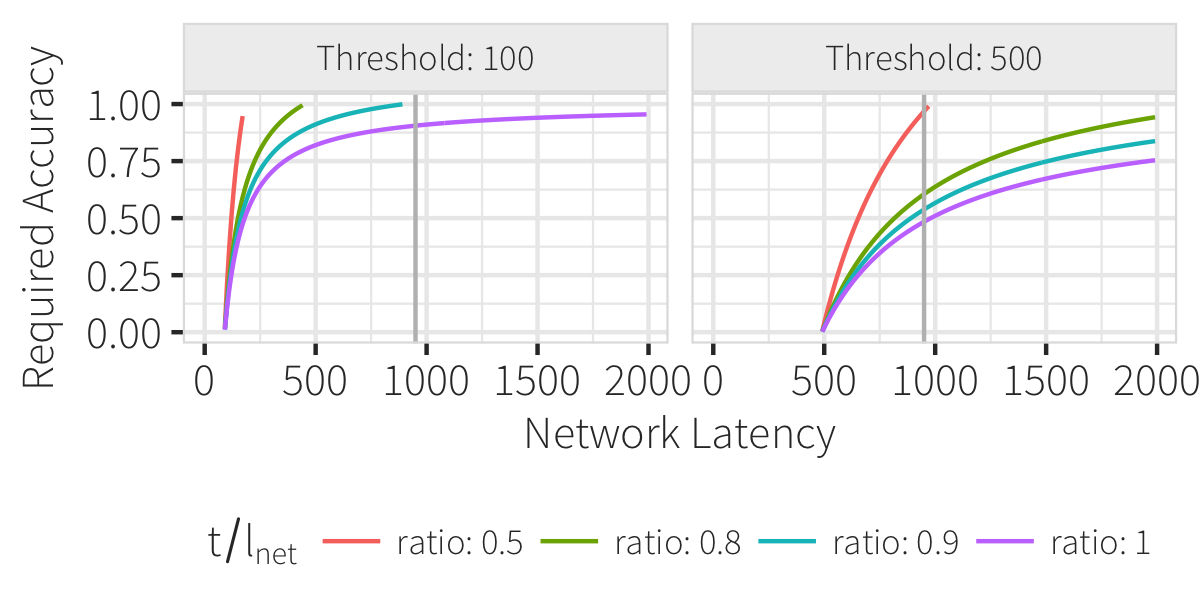
\includegraphics[width=1\columnwidth]{figures/model_base}
 	\caption{Minimum $\alpha$ vs network latency (x-axis), $\frac{t}{l_{net}}$ ratios (lines), and two thresholds (facets).}
    \label{fig:model_base}
\end{figure}



\stitle{Vary Prefetch Concurrency}
Most modern data processing systems are able to execute multiple concurrent requests~\cite{ebenstein2016fluxquery,giannikis2012shareddb}, thus we now modify the model to vary the number of concurrent prefetch requests $N$.
The $(1-\alpha)^N$ term is the probability that none of the prefetch requests match the user's actual request at $T=t$:
%
$$l_{user} = (l_{cache} + max(0, l_{net} - t)\times (1-(1-\alpha)^N) + l_{net}\times(1-\alpha)^N $$
%
Rearranging the terms results in the following minimum prediction accuracy:
%
$$\alpha = 1 - \left(\frac{l_{cache}+max(0,l_{net}-t)-l_{user}}{max(0,l_{net}-t)-l_{net}}\right)^{1/N}$$

\begin{figure}[h]
	\centering
	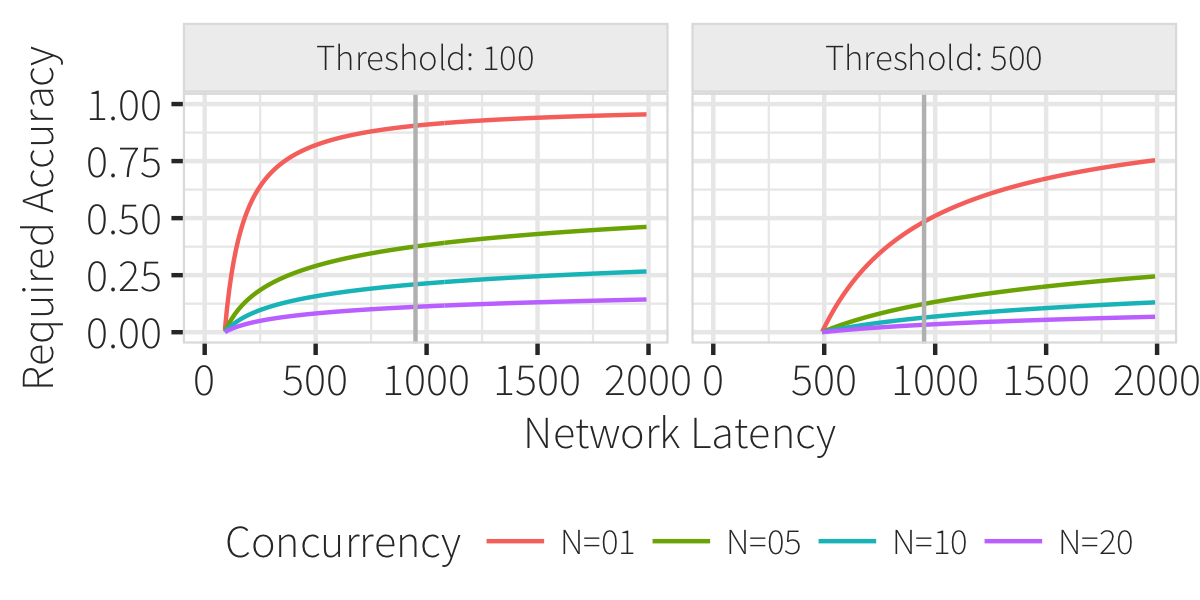
\includegraphics[width=1\columnwidth]{figures/model_concurrency}
 	\caption{Minimum $\alpha$ vs network latency (x-axis), concurrency (lines), and two latency thresholds (facets).}
  \label{fig:model_concurrency}
\end{figure}


Figure~\ref{fig:model_concurrency} shows that increasing the number of concurrent requests has an immediate effect on $\alpha$ ($t=l_{net}$ in these plots).    With $N=20$, a prediction model need only be $12\%$ accurate to ensure an interactive latency of $l_{user}=100$, while ensuring  $l_{user}=500$ only requires an accuracy of $3.5\%$.  At the limit, sending concurrent requests for all possible queries (assuming the cost is $l_{net}$) means the user latency is independent of prediction accuracy.  These results suggest that increasing the concurrency is an effective counter balance to model accuracy.


\stitle{Network Latency Variance}
Figure~\ref{fig:model_std} simulates $l_{net}$ drawn from a gaussian distribution with standard deviation of $std \in \{0, 100, 500\}$ milliseconds.  We set $N=20$, $t=l_{net}$, and the y-axis is from 0 to $0.4$.  Although the request variance affects the required model accuracy when $l_{net}$ is low, the curves for each threshold converge to the same levels independent of $std$; this is simply because $l_{net}$, rather than $std$, is the dominant factor as it increases.

\begin{figure}[h]
	\centering
	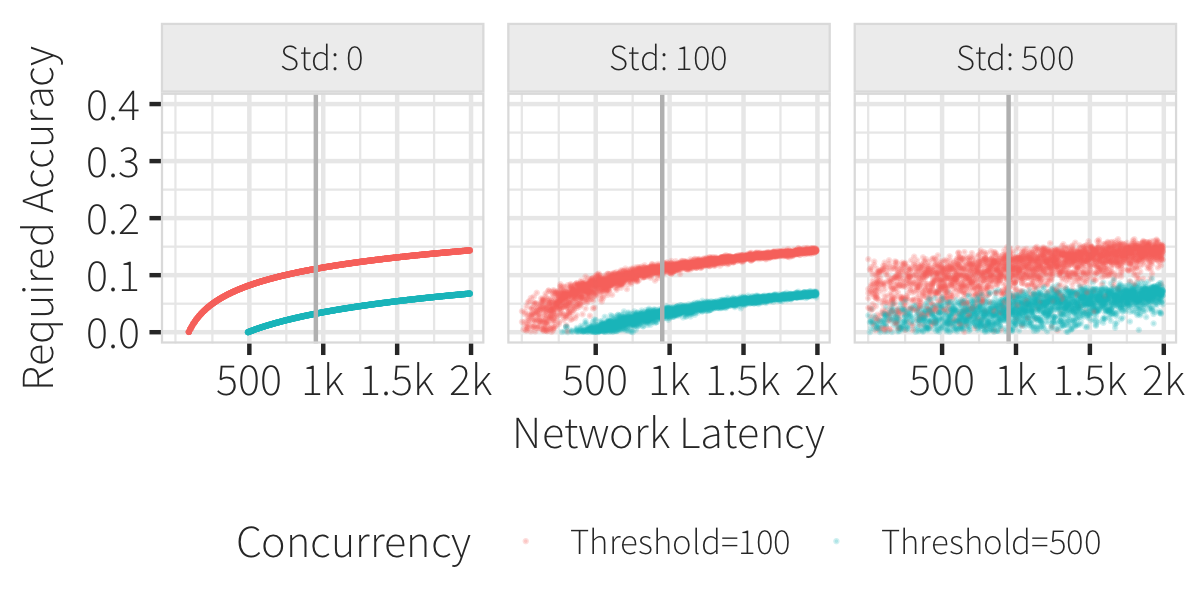
\includegraphics[width=1\columnwidth]{figures/model_std}
 	\caption{Minimum $\alpha$ vs network latency (x-axis), concurrency (lines), and two latency thresholds (facets).}
  \label{fig:model_std}
\end{figure}

\begin{figure}[h]
	\centering
	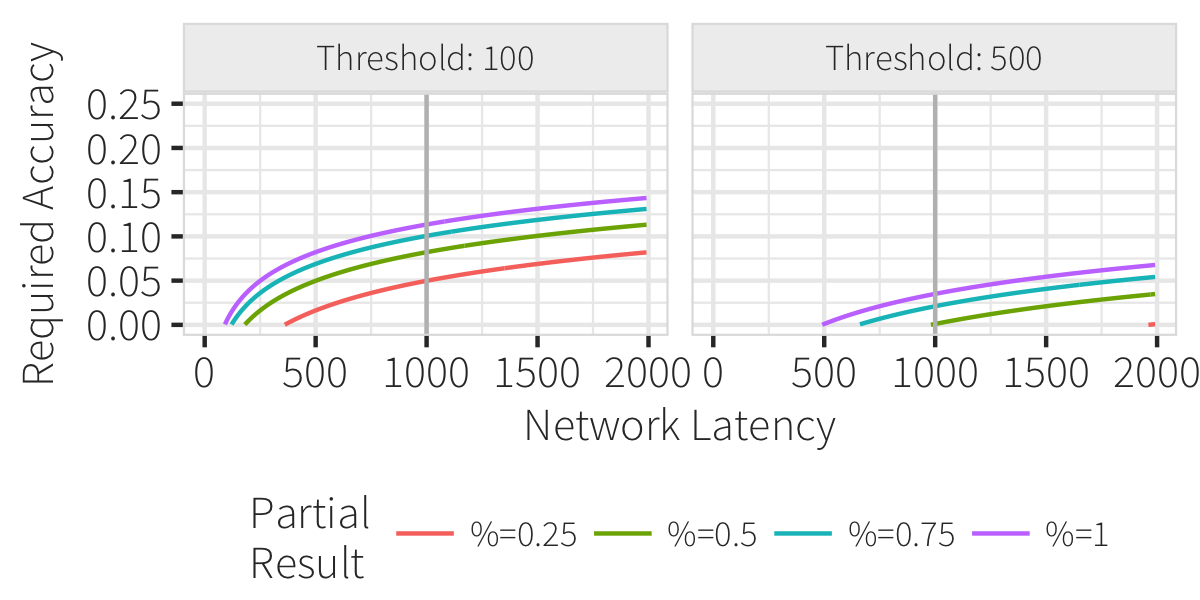
\includegraphics[width=1\columnwidth]{figures/model_partial}
 	\caption{Required prediction accuracy as a function of network latency, under progressive conditions where partial responses are sufficient.}
    \label{fig:model_partial}
\end{figure}


\stitle{Progressive Results}
The visualization and database communities have argued for approximate visualizations that are slightly inaccurate but potentially much faster to compute.  Techniques such as Online Aggergation~\cite{control,wanderjoin} or streaming wavelet compression~\cite{} are considered {\it progressive} because they are able to immediately return (and render) approximate results that improve over time; thus providing a natural trade-off between latency and result quality.  Our final analysis studies progressive results that require a fraction of the full request latency to be ``sufficiently good''.
\ewu{Use sampling and immens arguments as basis for 25\% partial results.} We find that $5\%$ accuracy is enough to maintain user perceived latency of $100$ when $25\%$ of the results is sufficient; at threshold of $500$, the perceived latency is independent of the model accuracy when $l_{net}\le 2000$.






\subsection{Discussion}
We find that a careful combination of existing techniques (concurrency and progressive results) can dramatically reduce the required model accuracy to enable low user perceived latency---in some extreme cases when the threshold is $500$, the model accuracy can even be $0\%$.  
\ewu{Argue that given  fixed network throughput between client and server, increasing concurrency beyond a certain point naturally requires partial results.  Thus the two go hand in hand.   We also see that the prediction model simply needs to be ``good enough'' with an accuracy of $5-10\%$.  When the number of possible interactions are limited to $10-20$ possible interactions, then even a random model is sufficient.  However in rich interfaces with potentially dozens or a hundred possible interactions, there may simply be too many choices to learn a good model.}

